\chapter{場景模擬}
\renewcommand{\baselinestretch}{10.0} %設定行距
\pagenumbering{arabic} %設定頁號阿拉伯數字
\setcounter{page}{17}  %設定頁數
\fontsize{14pt}{2.5pt}\sectionef
\section{摘要}
  完成球員及程式碼設定後,接著建立模擬場景,添加場地、球員、計時器、 LED 記分板和機械式轉盤記分板等等...。\\
\section{機械記分板放入場景}
  在 Coppeliasim 中導入 STL 圖檔,調整到合適方向,分別炸開物件,將數字部分調整成紅色,方便觀看。\\
\begin{figure}[hbt!]
\begin{center}
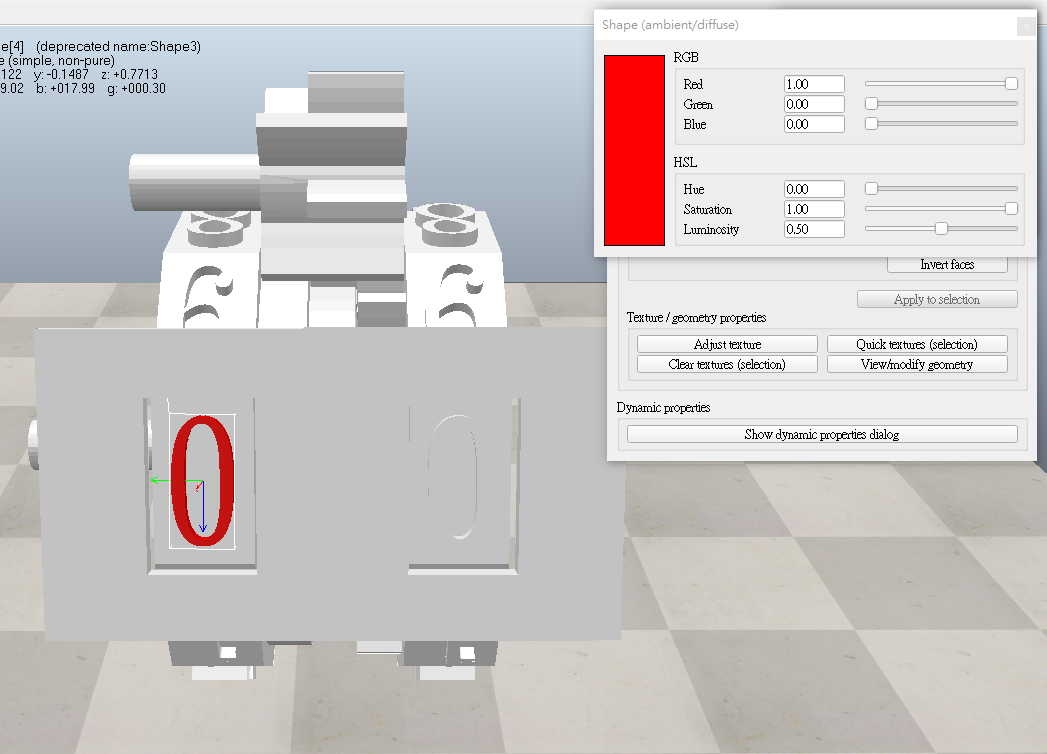
\includegraphics[height=6cm]{15}
\caption{\Large 數字調整顏色}\label{fig.15}
\end{center}
\end{figure}

  加入 joint 關節讓齒輪運轉,調整方位後依附在齒輪的中心軸上,除了主動軸外其他軸也要設定轉速為 0 ,避免模擬時齒輪隨意偏擺。\\
\begin{figure}[hbt!]
\begin{center}
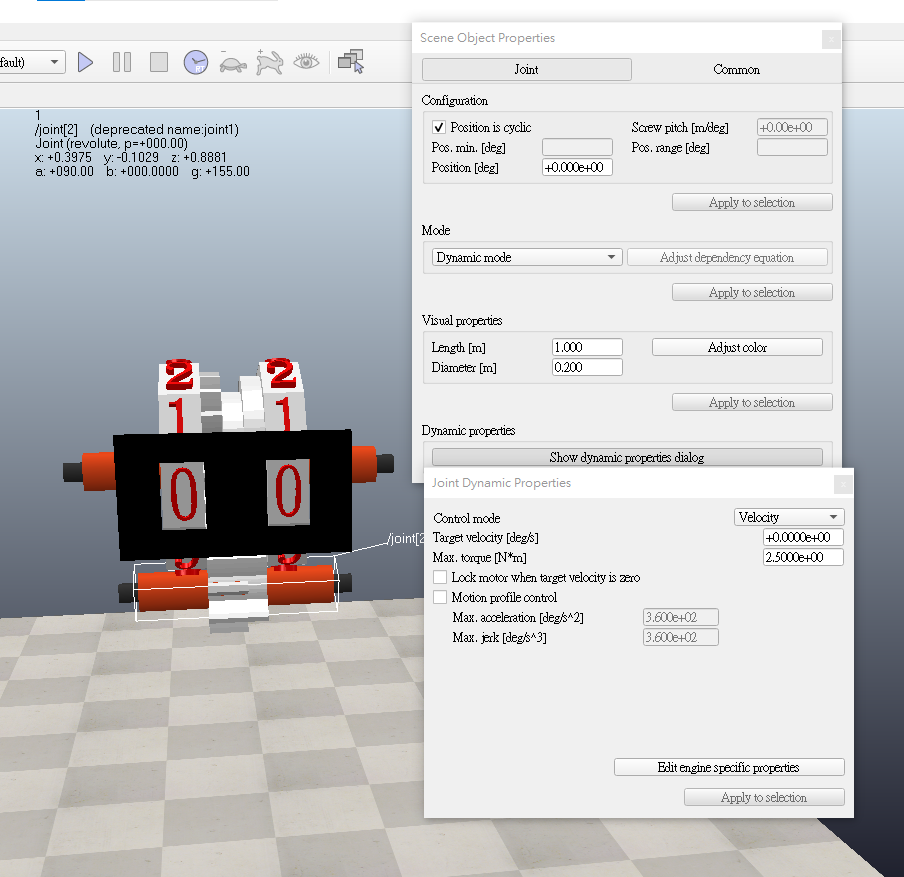
\includegraphics[height=6cm]{28}
\caption{\Large 設定轉速}\label{fig.28}
\end{center}
\end{figure}
\newpage
  調整質量及慣性矩後,記分板即可順利運轉。\\
\begin{figure}[hbt!]
\begin{center}
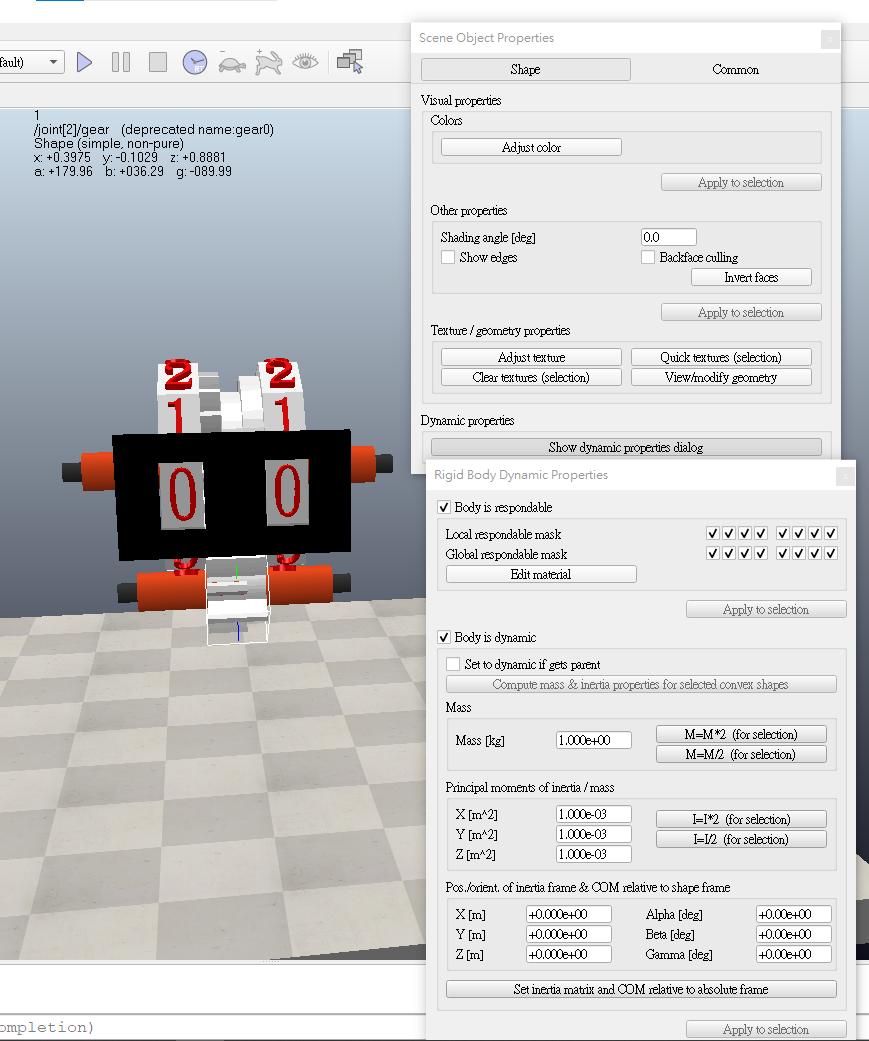
\includegraphics[height=6cm]{29}
\caption{\Large 給定質量}\label{fig.29}
\end{center}
\end{figure}

\newpage
\section{統整場景}
  在球場周圍設置空氣牆,放入 8 名球員,以兩色分為兩隊。\\
\begin{figure}[hbt!]
\begin{center}
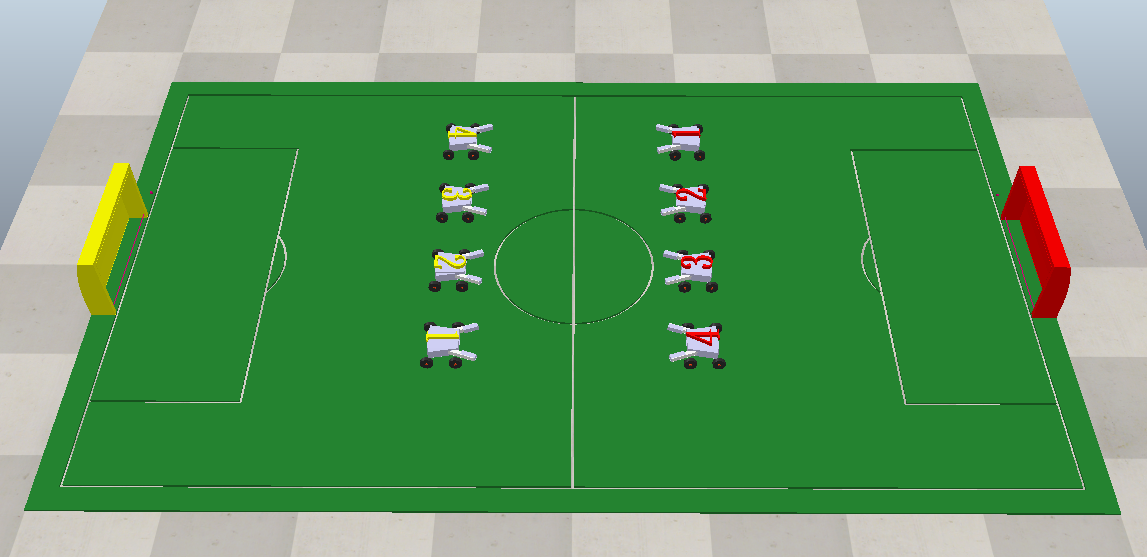
\includegraphics[height=6cm]{60}
\caption{\Large 球場建立}\label{fig.60}
\end{center}
\end{figure}

  以及計時器、LED計分板和機械式記分板。\\
\begin{figure}[hbt!]
\begin{center}
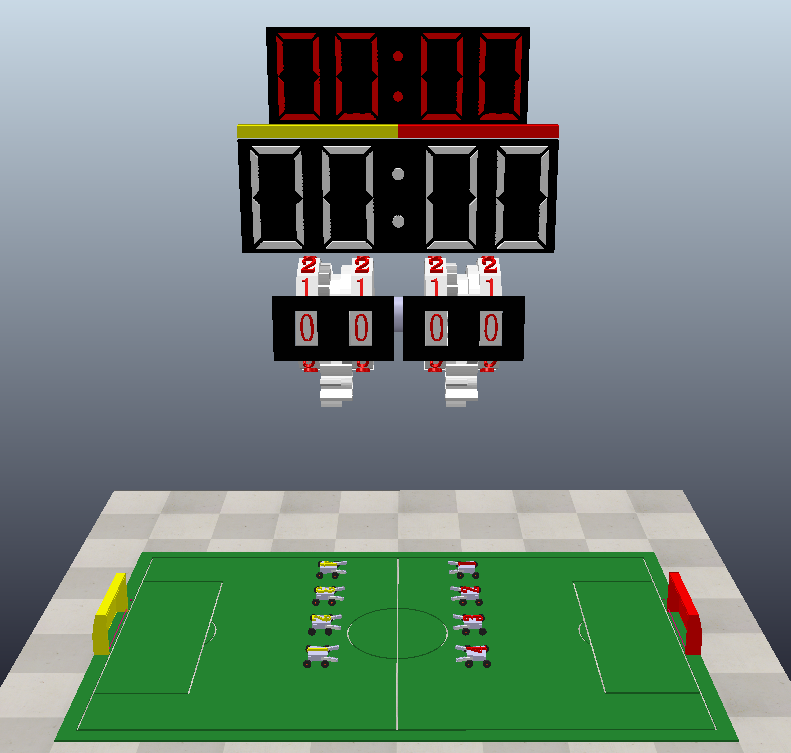
\includegraphics[height=10cm]{61}
\caption{\Large 球場全貌}\label{fig.61}
\end{center}
\end{figure}
\renewcommand{\baselinestretch}{1} %設定行距